\documentclass[10pt,aspectratio=169]{beamer}

\usepackage{booktabs}
\usepackage{tabularx}
\usepackage{array}
\usepackage{xcolor}
\usepackage{graphicx}
\usepackage{amsmath}

\graphicspath{{figures/}{report/figures/}}

\definecolor{DeepNavy}{HTML}{16324F}
\definecolor{SoftBlue}{HTML}{4F7CAC}
\definecolor{FreshTeal}{HTML}{3AAFA9}
\definecolor{WarmGray}{HTML}{F3F6F8}
\definecolor{Ink}{HTML}{1F2933}
\definecolor{Muted}{HTML}{657786}

\usetheme{Madrid}
\usecolortheme{default}
\setbeamertemplate{navigation symbols}{}
\setbeamertemplate{footline}[frame number]
\setbeamertemplate{blocks}[rounded][shadow=false]

\setbeamercolor{normal text}{fg=Ink,bg=white}
\setbeamercolor{title}{fg=white,bg=DeepNavy}
\setbeamercolor{frametitle}{fg=white,bg=DeepNavy}
\setbeamercolor{structure}{fg=SoftBlue}
\setbeamercolor{block title}{fg=white,bg=SoftBlue}
\setbeamercolor{block body}{fg=Ink,bg=WarmGray}
\setbeamercolor{alerted text}{fg=FreshTeal}

\setbeamerfont{title}{series=\bfseries,size=\Large}
\setbeamerfont{frametitle}{series=\bfseries}
\setbeamerfont{section in toc}{series=\bfseries}

\newcommand{\key}[1]{\textbf{\textcolor{FreshTeal}{#1}}}
\newcommand{\muted}[1]{{\scriptsize\textcolor{Muted}{#1}}}
\newcommand{\stagebox}[2]{%
    \fcolorbox{SoftBlue}{WarmGray}{%
        \begin{minipage}[t][0.34\textheight][t]{0.89\linewidth}
            \vspace{0.2em}
            \textbf{\textcolor{DeepNavy}{#1}}\par\vspace{0.3em}
            #2
        \end{minipage}%
    }%
}
\newcommand{\placeholderimage}[2]{%
    \fbox{%
        \begin{minipage}[c][#1][c]{0.92\linewidth}
            \centering
            \textcolor{Muted}{#2}
        \end{minipage}%
    }%
}

\title[StudyAssistant]{StudyAssistant: Retrieval-Augmented NLP System for Learning from Lecture PDFs}
\author{Member: [Your Name]}
\institute{Instructor: [Instructor Name]\\Natural Language Processing Project}
\date{\today}

\begin{document}

% 1
\begin{frame}
    \titlepage
    \vspace{-0.5em}
    \begin{center}
        \small Document-grounded search, answer generation, citation validation, and learning-material support.
    \end{center}
\end{frame}

% 2
\begin{frame}{Presentation Roadmap}
    \tableofcontents
\end{frame}

\section{System Overview}

% 3
\begin{frame}{System Architecture Overview}
    \begin{columns}[T,totalwidth=\textwidth]
        \begin{column}{0.58\textwidth}
            \IfFileExists{figures/full_pipeline.png}{%
                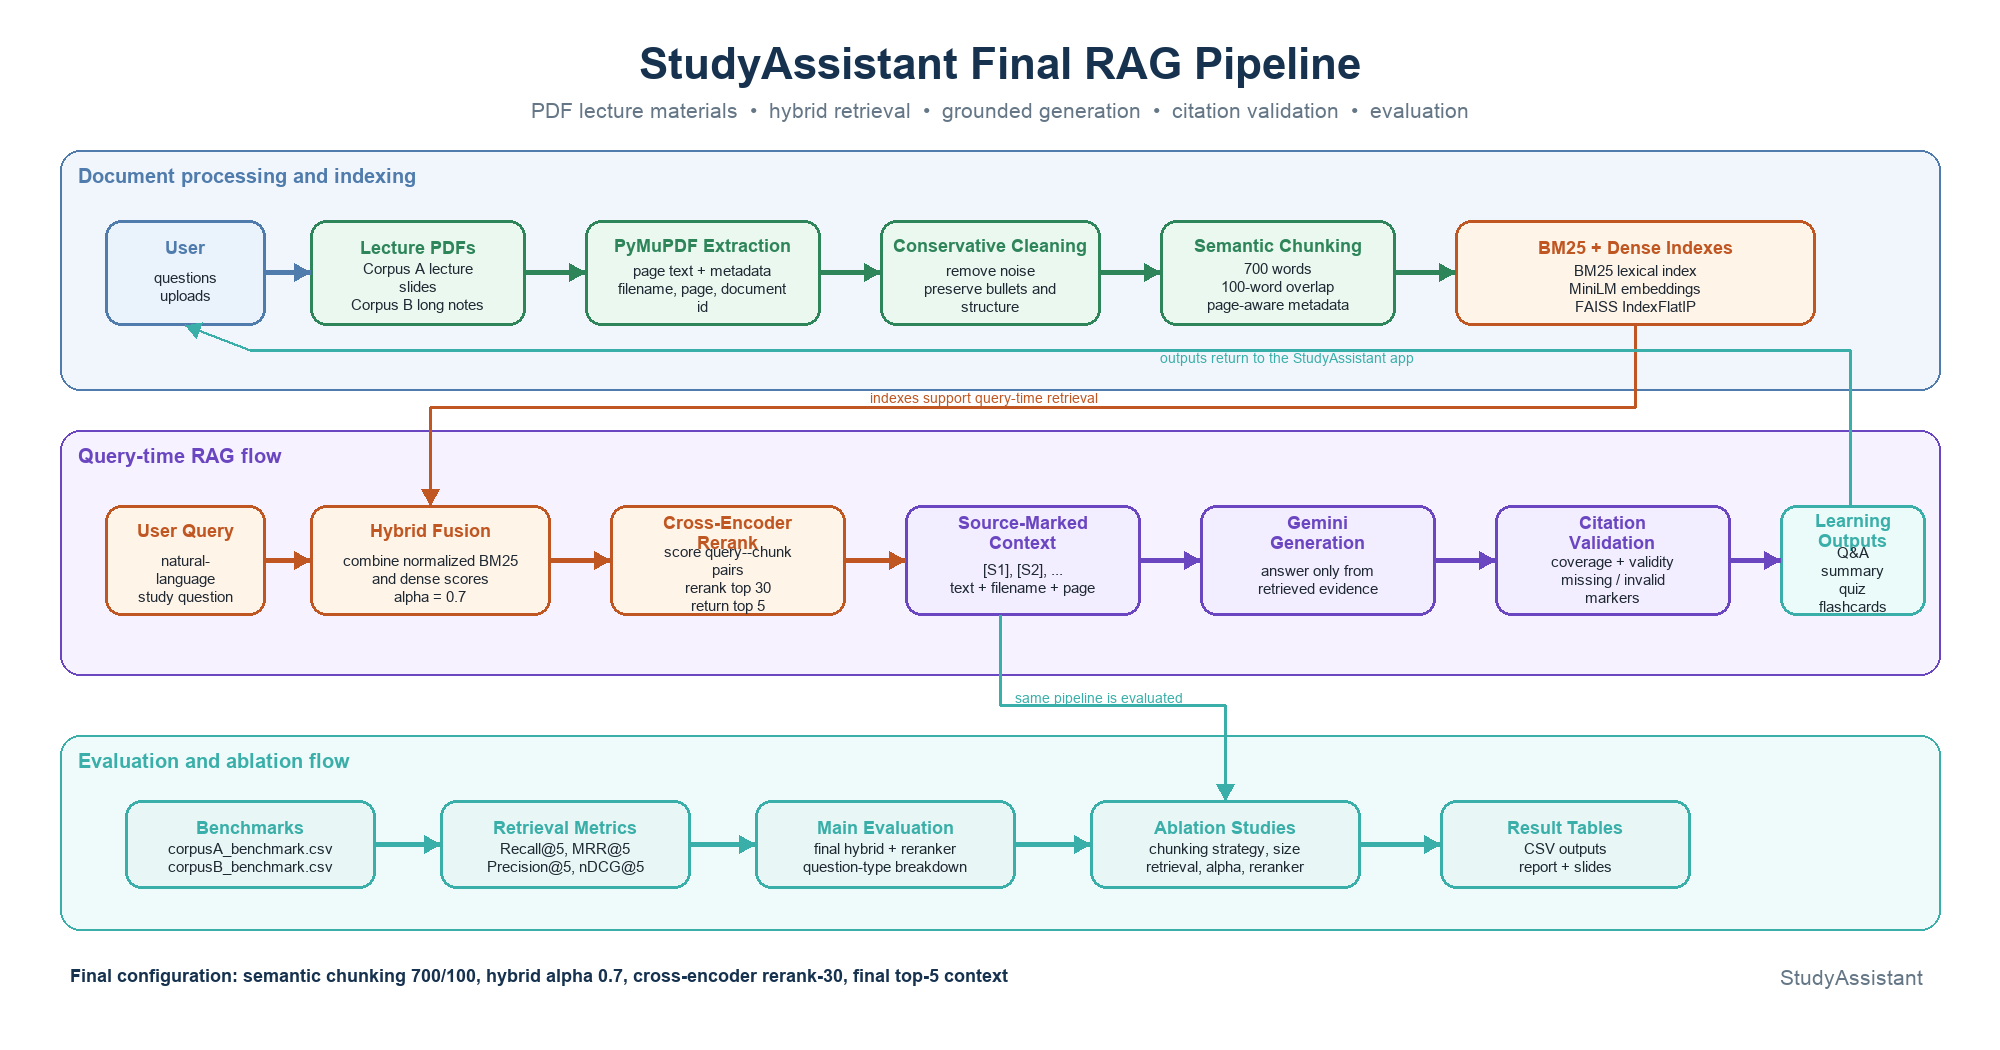
\includegraphics[width=\linewidth,height=0.72\textheight,keepaspectratio]{figures/full_pipeline.png}
            }{%
                \IfFileExists{report/figures/full_pipeline.png}{%
                    
\includegraphics[width=\linewidth,height=0.72\textheight,keepaspectratio]{report/figures/full_pipeline.png}
                }{%
                    \placeholderimage{0.56\textheight}{Pipeline image: PDF extraction $\rightarrow$ retrieval $\rightarrow$ reranking $\rightarrow$ generation}
                }%
            }
        \end{column}
        \begin{column}{0.38\textwidth}
            \textbf{Core idea}
            \begin{itemize}
                \item Convert PDFs into page-aware chunks.
                \item Retrieve evidence with BM25 + dense FAISS.
                \item Fuse and rerank candidate chunks.
                \item Generate answers with valid source markers.
            \end{itemize}
            \vspace{0.4em}
            \muted{The pipeline keeps filename, page, and chunk metadata from extraction to citation validation.}
        \end{column}
    \end{columns}
\end{frame}

\section{Methodology}

% 4
\begin{frame}{Document Extraction, Cleaning, and Chunking}
    \begin{columns}[T,totalwidth=\textwidth]
        \begin{column}{0.47\textwidth}
            \textbf{PDF extraction}
            \begin{itemize}
                \item PyMuPDF extracts text page by page.
                \item Each page keeps \texttt{document\_id}, filename, page number, and text.
            \end{itemize}

            \textbf{Cleaning}
            \begin{itemize}
                \item Conservative structure-preserving cleaning.
                \item Removes noise while keeping bullets, line breaks, and lecture structure.
            \end{itemize}
        \end{column}
        \begin{column}{0.49\textwidth}
            \textbf{Chunking design}
            \begin{itemize}
                \item Chunks are retrieval units, but metadata remains page-aware for citations.
                \item Default method: \key{semantic chunking}; compared with naive word-window and paragraph-aware chunking.
                \item Final configuration: \key{700 words} with \key{100-word overlap}.
                \item Overlap reduces boundary loss when definitions or examples cross chunk boundaries.
                \item Larger chunks preserve context but may introduce irrelevant text; smaller chunks are focused but may miss evidence.
            \end{itemize}
            \vspace{0.4em}
            \muted{Corpus B shows that 300-word chunks lose evidence, while 700/100 reaches the best MRR@5 and nDCG@5.}
        \end{column}
    \end{columns}
\end{frame}

% 5
\begin{frame}{Indexing, Hybrid Retrieval, and Reranking}
    \begin{columns}[T,totalwidth=\textwidth]
        \begin{column}{0.50\textwidth}
            \textbf{BM25 lexical indexing}
            \scriptsize
            \[
            s_{BM25}(q,d)=\sum_{t\in q} IDF(t)
            \frac{f(t,d)(k_1+1)}
            {f(t,d)+k_1(1-b+b\frac{|d|}{avgdl})}
            \]
            \normalsize
            \begin{itemize}
                \item Strong for exact terms in lecture slides.
                \item Handles term frequency and document-length normalization.
            \end{itemize}
        \end{column}
        \begin{column}{0.46\textwidth}
            \textbf{Dense indexing and reranking}
            \scriptsize
            \[
                e_q=\frac{Enc(q)}{\|Enc(q)\|}, \quad
                e_d=\frac{Enc(d)}{\|Enc(d)\|}, \quad
                s_{dense}=e_q^\top e_d
            \]
            \normalsize
            \begin{itemize}
                \item FAISS \texttt{IndexFlatIP} stores normalized chunk vectors.
                \item Hybrid fusion uses $score=\alpha s_{dense}+(1-\alpha)s_{BM25}$.
                \item Cross-encoder reranks the initial candidate pool.
            \end{itemize}
        \end{column}
    \end{columns}
    \vspace{0.4em}
    \centering
    \muted{Final settings: $\alpha=0.7$, rerank top 30 candidates to final top 5.}
\end{frame}

% 6
\begin{frame}{Generation, Citation Validation, and Study Outputs}
    \begin{columns}[T,totalwidth=\textwidth]
        \begin{column}{0.32\textwidth}
            \stagebox{Context Construction}{
                \begin{itemize}\scriptsize
                    \item Top-5 chunks become source-marked context.
                    \item Markers such as \texttt{[S1]} map to file and page.
                    \item Metadata is kept for traceability.
                \end{itemize}
            }
        \end{column}
        \begin{column}{0.32\textwidth}
            \stagebox{Grounded Generation}{
                \begin{itemize}\scriptsize
                    \item Gemini answers only from retrieved context.
                    \item The prompt asks the model to refuse unsupported questions.
                    \item Factual claims should include source markers.
                \end{itemize}
            }
        \end{column}
        \begin{column}{0.32\textwidth}
            \stagebox{Validation and Outputs}{
                \begin{itemize}\scriptsize
                    \item Citation coverage and marker validity.
                    \item Summary generation.
                    \item Quiz and flashcard generation with JSON checks.
                \end{itemize}
            }
        \end{column}
    \end{columns}
    \vspace{0.7em}
    \centering
    \textcolor{SoftBlue}{Evidence} $\rightarrow$
    \textcolor{SoftBlue}{source markers} $\rightarrow$
    \textcolor{SoftBlue}{grounded answer} $\rightarrow$
    \textcolor{SoftBlue}{validation}
\end{frame}

\section{Evaluation}

% 7
\begin{frame}{Evaluation Setup: Corpora, Benchmarks, and Runs}
    \begin{columns}[T,totalwidth=\textwidth]
        \begin{column}{0.48\textwidth}
            \textbf{Corpus A: lecture slides}
            \begin{itemize}
                \item 9 NLP lecture PDFs.
                \item 120 benchmark questions.
                \item 100 answerable questions used for retrieval metrics.
                \item 20 unanswerable questions reserved for answerability evaluation.
            \end{itemize}
        \end{column}
        \begin{column}{0.48\textwidth}
            \textbf{Corpus B: long document}
            \begin{itemize}
                \item \texttt{DL\_LectureNotes.pdf}.
                \item 35 answerable questions with page-level gold sources.
                \item Used for chunking strategy and chunk-size robustness.
                \item Page-level relevance uses \texttt{filename:page}.
            \end{itemize}
        \end{column}
    \end{columns}
    \vspace{0.6em}
    \textbf{Default run:} semantic chunking, 700/100 chunks, BM25 + dense FAISS,
    hybrid min-max fusion, $\alpha=0.7$, rerank-30, final top-5.
\end{frame}

% 8
\begin{frame}{Evaluation Metrics}
    \begin{columns}[T,totalwidth=\textwidth]
        \begin{column}{0.48\textwidth}
            \textbf{Retrieval metrics}
            \begin{itemize}
                \item \key{Recall@5}: whether gold evidence appears in the retrieved context.
                \item \key{MRR@5}: rank of the first relevant result.
                \item \key{Precision@5}: fraction of retrieved chunks counted as relevant.
                \item \key{nDCG@5}: ranking quality with position discounting.
                \item \key{Latency}: mean retrieval time per query.
            \end{itemize}
        \end{column}
        \begin{column}{0.48\textwidth}
            \textbf{Generation and validation metrics}
            \begin{itemize}
                \item Exact Match and Token F1 compare generated and reference answers.
                \item Answerability accuracy checks refusal on unanswerable questions.
                \item Citation coverage checks whether answers cite sources.
                \item Citation validity checks whether markers exist in context.
                \item Learning outputs use JSON, structure, duplicate, and grounding checks.
            \end{itemize}
        \end{column}
    \end{columns}
\end{frame}

% 9
\begin{frame}{Main Results: Final Retrieval}
    \begin{columns}[T,totalwidth=\textwidth]
        \begin{column}{0.50\textwidth}
            \textbf{Corpus A final pipeline}
            \small
            \begin{tabular}{lcc}
                \toprule
                Metric & Score & Notes \\
                \midrule
                Recall@5 & \textbf{0.890} & evidence coverage \\
                MRR@5 & \textbf{0.788} & early rank \\
                Precision@5 & 0.178 & single-page labels \\
                nDCG@5 & \textbf{0.814} & ranking quality \\
                Latency & 490.1 ms & rerank enabled \\
                \bottomrule
            \end{tabular}
            \vspace{0.2em}
        \end{column}
        \begin{column}{0.48\textwidth}
            \textbf{Question-type breakdown}
            \scriptsize
            \begin{tabular}{lcccc}
                \toprule
                Type & Recall & MRR & Prec. & nDCG \\
                \midrule
                Comparison & \textbf{1.000} & \textbf{1.000} & 0.200 & \textbf{1.000} \\
                Definition & \textbf{0.962} & 0.847 & 0.192 & 0.876 \\
                Explanation & 0.750 & 0.688 & 0.150 & 0.704 \\
                Factual & 0.821 & 0.713 & 0.164 & 0.740 \\
                \bottomrule
            \end{tabular}
            \vspace{0.5em}
            \normalsize
            \textbf{Analysis}
            \begin{itemize}
                \item Relevant evidence appears in top-5 for 89\% of questions.
                \item Definitions benefit from exact lecture terminology.
                \item Explanation questions are harder because phrasing differs from slides.
            \end{itemize}
        \end{column}
    \end{columns}
\end{frame}

\section{Ablation Study}

% 10
\begin{frame}{Ablation Study: Chunking}
    \begin{columns}[T,totalwidth=\textwidth]
        \begin{column}{0.56\textwidth}
            \textbf{Chunk-size ablation on Corpus B}
            \scriptsize
            \begin{tabular}{ccccc}
                \toprule
                Size & Overlap & Recall@5 & MRR@5 & nDCG@5 \\
                \midrule
                300 & 50 & 0.457 & 0.314 & 0.350 \\
                500 & 80 & \textbf{0.657} & 0.380 & 0.448 \\
                700 & 100 & \textbf{0.657} & \textbf{0.396} & \textbf{0.461} \\
                1000 & 150 & \textbf{0.657} & \textbf{0.396} & \textbf{0.461} \\
                1500 & 200 & \textbf{0.657} & \textbf{0.396} & \textbf{0.461} \\
                \bottomrule
            \end{tabular}
            \vspace{0.7em}
            \textbf{Chunking strategy}
            \scriptsize
            \begin{tabular}{lccc}
                \toprule
                Strategy & Chunks & Recall@5 & nDCG@5 \\
                \midrule
                Naive & 190 & \textbf{0.657} & \textbf{0.461} \\
                Paragraph & 190 & \textbf{0.657} & \textbf{0.461} \\
                Semantic & 190 & \textbf{0.657} & \textbf{0.461} \\
                \bottomrule
            \end{tabular}
        \end{column}
        \begin{column}{0.40\textwidth}
            \textbf{Analysis}
            \begin{itemize}
                \item 300-word chunks are too small and lose evidence.
                \item 700/100 gives the best MRR@5 and nDCG@5 while keeping context controlled.
                \item Strategy scores are equal because the long document is processed page-preservingly.
                \item Final configuration keeps semantic chunking for robustness.
            \end{itemize}
        \end{column}
    \end{columns}
\end{frame}

% 11
\begin{frame}{Ablation Study: Retrieval, Alpha, and Reranking}
    \begin{columns}[T,totalwidth=\textwidth]
        \begin{column}{0.60\textwidth}
            \scriptsize
            \textbf{Retrieval component}
            \begin{tabular}{lccc}
                \toprule
                Method & Recall & MRR & nDCG \\
                \midrule
                BM25 & 0.700 & 0.581 & 0.611 \\
                Dense & 0.690 & 0.490 & 0.539 \\
                Hybrid & \textbf{0.830} & \textbf{0.660} & \textbf{0.703} \\
                \bottomrule
            \end{tabular}

            \vspace{0.6em}
            \textbf{Hybrid alpha}
            \begin{tabular}{lccc}
                \toprule
                $\alpha$ & Recall & MRR & nDCG \\
                \midrule
                0.0 & 0.700 & 0.581 & 0.611 \\
                0.5 & 0.790 & 0.641 & 0.679 \\
                0.7 & \textbf{0.830} & 0.660 & \textbf{0.703} \\
                1.0 & 0.690 & 0.490 & 0.539 \\
                \bottomrule
            \end{tabular}

            \vspace{0.6em}
            \textbf{Reranking}
            \begin{tabular}{lccc}
                \toprule
                Setting & Recall & MRR & nDCG \\
                \midrule
                None & 0.830 & 0.660 & 0.703 \\
                Top 10 & 0.840 & 0.759 & 0.779 \\
                Top 30 & \textbf{0.890} & \textbf{0.788} & \textbf{0.814} \\
                Top 50 & 0.880 & 0.785 & 0.809 \\
                \bottomrule
            \end{tabular}
        \end{column}
        \begin{column}{0.36\textwidth}
            \textbf{Analysis}
            \begin{itemize}
                \item Hybrid combines exact lecture terms and semantic matching.
                \item $\alpha=0.7$ gives the best Recall@5 and nDCG@5.
                \item Reranking improves ranking by directly scoring query--chunk pairs.
                \item Rerank-50 is slower and does not improve quality over rerank-30.
            \end{itemize}
        \end{column}
    \end{columns}
\end{frame}

\section{Demo and Conclusion}

% 12
\begin{frame}{Demo: Streamlit Study Assistant}
    \begin{columns}[T,totalwidth=\textwidth]
        \begin{column}{0.62\textwidth}
            \IfFileExists{figures/app_screenshot.png}{%
                \includegraphics[width=\linewidth,height=0.72\textheight,keepaspectratio]{figures/app_screenshot.png}
            }{%
                \IfFileExists{report/figures/app_screenshot.png}{%
                    \includegraphics[width=\linewidth,height=0.72\textheight,keepaspectratio]{report/figures/app_screenshot.png}
                }{%
                    \placeholderimage{0.62\textheight}{Add app screenshot at \texttt{report/figures/app\_screenshot.png}}
                }%
            }
        \end{column}
        \begin{column}{0.34\textwidth}
            \textbf{Demo workflow}
            \begin{enumerate}
                \item Upload lecture PDFs.
                \item Ask a natural-language question.
                \item Inspect retrieved sources.
                \item Generate cited answer.
                \item Create quiz or flashcards.
            \end{enumerate}
            \vspace{0.5em}
            \muted{Run locally with: \texttt{streamlit run app.py}}
        \end{column}
    \end{columns}
\end{frame}

% 13
\begin{frame}{Conclusion and Future Work}
    \textbf{Key findings}
    \begin{itemize}
        \item Final retrieval reaches \key{0.890 Recall@5} and \key{0.814 nDCG@5}.
        \item Hybrid retrieval outperforms BM25-only and dense-only baselines.
        \item Rerank-30 is the best quality setting for the final pipeline.
        \item 700/100 chunking is more reliable than very small chunks on Corpus B.
        \item Citation validation catches marker-level citation failures.
    \end{itemize}

    \vspace{0.6em}
    \textbf{Future work}
    \begin{itemize}
        \item Add chunk-level gold labels and more balanced question types.
        \item Run full Gemini generation evaluation with manual groundedness labels.
        \item Add OCR/layout-aware extraction for figures, tables, and scanned slides.
        \item Tune interactive speed/accuracy modes for reranking.
    \end{itemize}

    \vfill
    \begin{center}
        \Large \textcolor{DeepNavy}{Thank you}
    \end{center}
\end{frame}

\end{document}
